\documentclass[conference]{IEEEtran}
\usepackage[english]{babel}
\usepackage{cite,setspace}
\usepackage[autostyle]{csquotes}
\usepackage{amsmath,amssymb,amsfonts}
\usepackage{algorithmic}
\usepackage{graphicx}
\graphicspath{{images/}}
\usepackage{textcomp}
\usepackage{xcolor}
\usepackage{float}
\restylefloat{table}
\restylefloat{figure}
\usepackage{subcaption}
\usepackage{changepage}
\usepackage{pgfplots}
\usepackage{tikz,tkz-euclide}
\usetikzlibrary{fadings}
\usepackage{siunitx}
\usepackage{pgfplots}
\usepackage[outputdir=output]{minted}
%\usemintedstyle{autumn} % friendly, colorful
%\newminted{c}{mathescape, linenos, numbersep=5pt, gobble=0, frame=lines, framesep=2mm}
%\definecolor{background}{gray}{0.90}
%\newminted{bash}{bgcolor=background}
%\newminted{console}{bgcolor=background}
%\usemintedstyle[console]{bw}
\def\BibTeX{{\rm B\kern-.05em{\sc i\kern-.025em b}\kern-.08em
    T\kern-.1667em\lower.7ex\hbox{E}\kern-.125emX}}
\captionsetup{width=.8\linewidth}

% Colors (RGB)=>(BRG)
% -------------------
%\definecolor{1,1,1}{RGB}{191,255,255}
\definecolor{8,8,8}{RGB}{3,24,96}
% R
\definecolor{0,0,0}{RGB}{255,255,255}
\definecolor{1,0,0}{RGB}{255,223,255}
\definecolor{6,0,0}{RGB}{255,127,255}
\definecolor{7,0,0}{RGB}{255,0,255}
% R + B
\definecolor{0,0,7}{RGB}{0,255,255}
%\definecolor{1,0,7}{RGB}{0,223,255}
\definecolor{6,0,7}{RGB}{0,127,255}
\definecolor{7,0,7}{RGB}{0,0,255}
% G
\definecolor{0,1,0}{RGB}{255,255,247}
\definecolor{0,2,0}{RGB}{255,255,223}
\definecolor{0,3,0}{RGB}{255,255,191}
\definecolor{0,4,0}{RGB}{255,255,153}
\definecolor{0,5,0}{RGB}{255,255,127}
\definecolor{0,6,0}{RGB}{255,255,63}
\definecolor{0,7,0}{RGB}{255,255,0}
% G + *
\definecolor{2,4,0}{RGB}{223,191,191}
\definecolor{0,4,2}{RGB}{191,255,191}
\definecolor{4,4,0}{RGB}{223,153,191}
\definecolor{0,4,4}{RGB}{153,255,191}
\definecolor{2,6,0}{RGB}{223,191,127}
\definecolor{0,6,2}{RGB}{191,255,127}
\definecolor{4,6,0}{RGB}{223,153,127}
\definecolor{0,6,4}{RGB}{153,255,127}
% G with gradient R + B
\definecolor{1,0,7}{RGB}{63,223,255}
\definecolor{1,1,7}{RGB}{32,223,223}
\definecolor{1,2,7}{RGB}{16,223,191}
\definecolor{1,3,7}{RGB}{0,223,153}
\definecolor{1,4,7}{RGB}{0,223,127}
\definecolor{1,5,7}{RGB}{0,191,63}
\definecolor{1,6,7}{RGB}{0,153,32}
\definecolor{1,7,7}{RGB}{0,127,16}
\definecolor{7,0,1}{RGB}{223,63,255}
\definecolor{7,1,1}{RGB}{223,32,223}
\definecolor{7,2,1}{RGB}{223,16,191}
\definecolor{7,3,1}{RGB}{223,0,153}
\definecolor{7,4,1}{RGB}{223,0,127}
\definecolor{7,5,1}{RGB}{191,0,63}
\definecolor{7,6,1}{RGB}{153,0,32}
\definecolor{7,7,1}{RGB}{127,0,16}

\pgfdeclarefading{rectangular fading}{
  \tikz {
    \shade [middle color=pgftransparent!0, left color=pgftransparent!0, top color=pgftransparent!100] (-2,2) -- (2,2) -- (2,-2) -- (-2,-2) -- cycle;
  }
}

\begin{document}

\title{Scene Semantics Applied to \\ Dynamic Frame Generation}

\author{\IEEEauthorblockN{Mark Wesley Harris}
\IEEEauthorblockA{\textit{CS5800 Computer Graphics, Fall 2019} \\
\textit{University of Colorado Colorado Springs}\\
Colorado Springs, United States \\
wharris2@uccs.edu}}

\maketitle

\begin{abstract}
% derp
\end{abstract}

\section{Introduction}
\label{sec:introduction}
Access to good training data is necessary
in order to harness the power of machine learning.
One such data to be studied is the relationship
between a 3D environment and the
rendered frame(s) it produces.
For the purposes of this document, this relationship is
referred to as the semantics of the given 3D scene --
i.e. the description of the 3D environment and its complexity
in relation to what is rendered.
This study is key to understanding and perhaps improving the
render pipeline and current rendering techologies.
However, extracting this data from the render process into a usable
format is not straightforward.

\section{Research}
We researched RenderMan for Maya (RfM) and concepts from Computer Graphics
that could help in determining scene semantics.
Of these concepts includes ray tracing, ray marching, and shaders.

\subsection{Ray Tracing and Ray Marching}
Ray tracing and ray marching in the context of RenderMan shaders were studied.
Figure \ref{fig:ray_marching} shows an example of how ray marching is applied to
create volumetric shaders, such as smoke or fog \cite{ray_marching}.
It was thought that these properties could be used to extract useful semantic data
during the rendering process.

Ray tracing is the study of how light behaves in a given environment.
Figure \ref{fig:raytrace}
shows a ray tracing problem studied in 1986, where light rays were mapped from
the viewer to a light source. Avro \textit{et al.}
discuss the difficulty of this problem,
as it involves taking into consideration material properties, light sources,
and where the viewer is looking \cite{backwards_raytrace}.

\begin{figure}[htbp]
\centerline{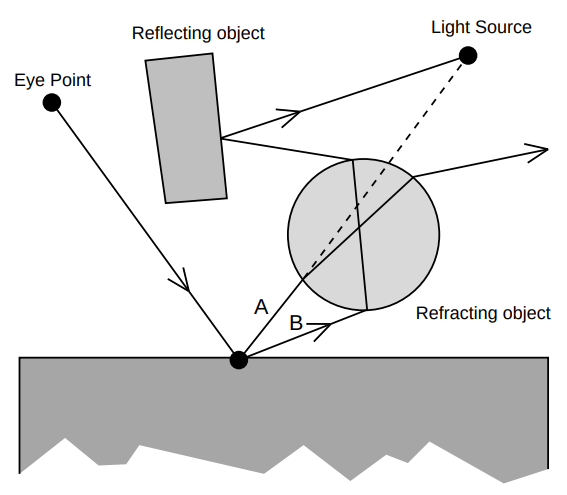
\includegraphics[width=5cm]{raytrace.png}}
\caption{Example of a problem in ray tracing \cite{backwards_raytrace}.}
\label{fig:raytrace}
\end{figure}

Technological advancements since 1986 have greatly improved ray tracing capabilities.
The ray tracing basics described by Scratchapixel 
provides a walkthrough with code samples for casting rays from the camera
\cite{raytrace_walkthrough}.

\begin{figure}[htbp]
\centering
{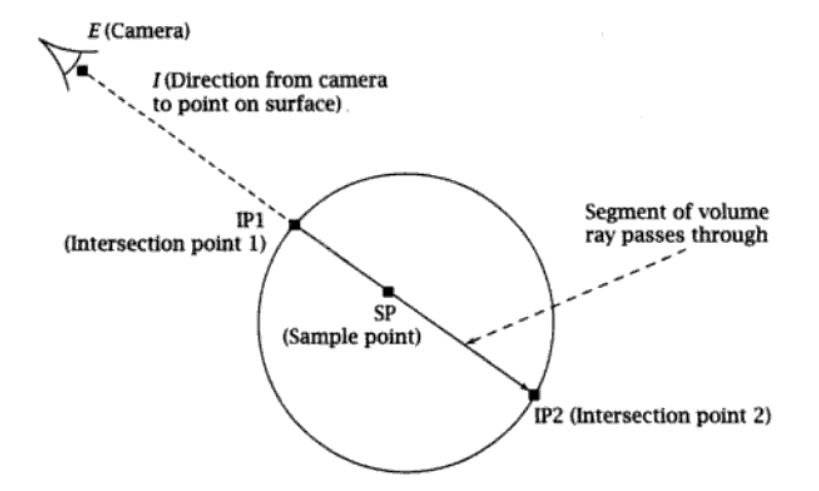
\includegraphics[width=7cm]{ray_marching.png}}
\caption{Ray marching technique for volumetric shading \cite{ray_marching}.}
\label{fig:ray_marching}
\end{figure}

\subsection{Shaders}
RenderMan includes many resources on shaders via their documentation,
however outside of officially produced sources there is a lack of any tutorials or
walkthroughs for shaders in the new RenderMan system.
Since RenderMan is maintained by Pixar Animation Studios and not a software solution
company, tutorials and walkthroughs were somewhat hard to find.
Introduction materials provided by Pixar were used to research the capabilities
of RenderMan shaders and the rendering pipeline \cite{renderman}.

Shaders are written in one of 3 ways: Patterns, Shading Language, and C++ \cite{shading}.
Patterns are useful for adding noise to shaders, or generating source data
programatically. This includes fractals, shapes, gradients, mult-layered noise,
which can be combined in different ways to create unique images.
Examples of this include rust, wavy glass, or vector-based shading.
Shading Language is a tool artists use to program shaders.
``RenderMan Shading Language (RSL) \dots includes math operations (sin, sqrt, etc.),
vector and matrix operations, coordinate transformations, and higher level functions like noise and texture''
\cite{renderman_docs}.
Shaders for RenderMan are written in RSL (a branch from OSL), or C++.

In any of the three cases, the shader outputs are not written directly
from shaders to the rendered image. They are applied to a BxDF material
(the base BxDF material for RenderMan is called ``PxrSurface''),
and data from all materials in the scene are combined and sent to an Integrator.
Integrators can be hot-swapped for different types of rendering and debugging of
shader code.
Upon researching how ray tracing is handled, we found that information
on refracted rays is passed
back to the BxDF for more sampling.
Anti-aliasing and other filters can be added at the end as necessary

\begin{figure}[htbp]
\centering
{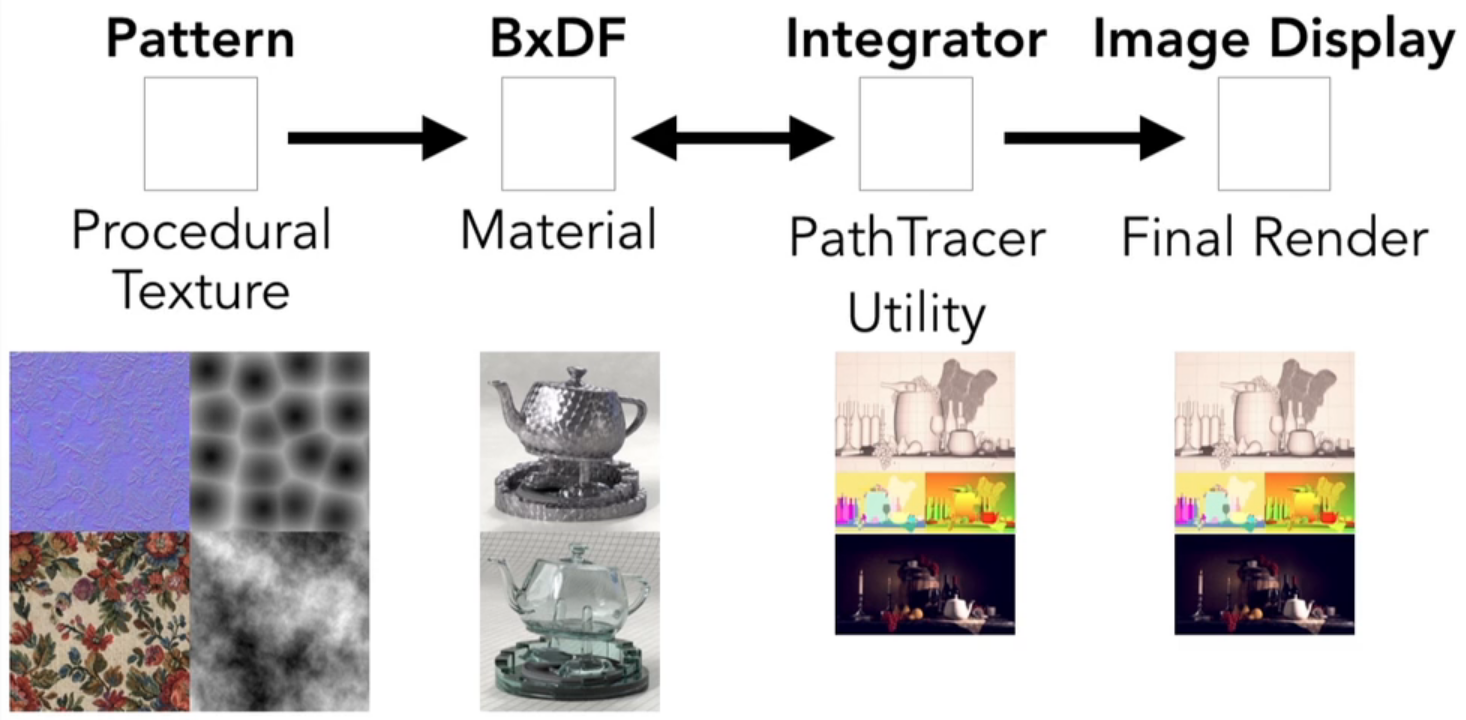
\includegraphics[width=7cm]{interaction.png}}
\caption{Data interactions between shaders and the rendered frame  \cite{renderman}.}
\label{fig:interaction}
\end{figure}

We found that shaders have complex interactions with data during ray tracing,
however it is unclear how to extract the data for later use.
A custom integrator could be written to collect the data, but even then it
may lose the connections with the scene that we require for semantics generation.
So, while the processes of ray tracing and ray marching have powerful capabilities,
we found it infeasible to extract the data they create during processing.
We discovered that, although using values from within the shaders is impractical,
we can take advantage of a shader's inputs and outputs to store the data we want to
use in our scene.
This approach disregards the use of ray tracing or ray marching,
but retains the concept of encoding data into the scene that can later be used
for generating semantics.

\section{Environment Setup}
Quality source material is key for a successful research project.
A powerful computer and complex animation source file are both required
for good research on this topic.
Described here are the steps taken for setting up the project
source materials and environment, as well as discussion on future steps
for how to use these sources for researching scene semantics.

\subsection{Computer Build}
A new computer was built at the start of the semester, in order to better prepare for the necessary machine learning
research and graphical image processing. One RTX 2060 GPU was purchased,
since the 2060 model is the cheapest GPU that also has Tensor cores
(which are useful specifically for training machine learning models).
The processor chosen was the AMD RYZEN 3600.
All the components were assembled,
and the result was a well-equipped computer running Windows 10 Pro.

\subsection{Rendering Technologies}
Two renderers that are now highly developed are the Arnold Renderer \cite{arnold}
and the RenderMan renderer \cite{renderman_docs}. Each of these renderers
function differently.
RenderMan 22 -- which is maintained by Pixar Animation Studios --
was chosen to be the renderer software for the purposes of this project,
since it is arguably the most advanced renderer developed to date.
The target platform was Autodesk Maya, and all Python scripts are unique to the
Maya environment.

The RenderMan Interface is proposed to be used as a gateway
into producing the bulk of scene semantics.
The RenderMan Interface provides implementations for rendering
``\dots hidden surfaces, spatial filtering, dithering, motion blur, depth of field,
flat and curved surfaces, objects, constructive solid geometry,
and programmable shading to express lighting conditions, shadows, and surface appearances,
with sophisticated control over color, texture, and reflectivity''
\cite{renderman_docs}.
Many of these attributes are out of scope
for this project, however they may later be explored in order to test the capabilities
of what is developed.
See Figure \ref{fig:renderman} for examples of dynamic scenes rendered with RenderMan.

\begin{figure}[htbp]
\centerline{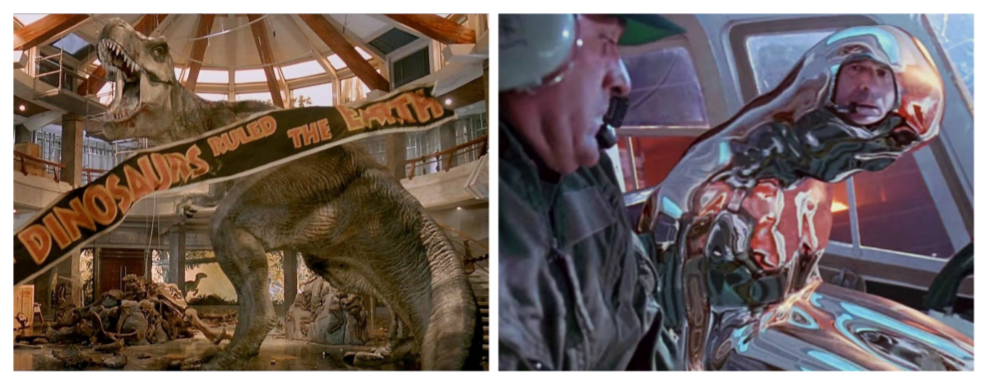
\includegraphics[width=8cm]{renderman.png}}
\caption{Path-traced images rendered with RenderMan \cite{renderman}.}
\label{fig:renderman}
\end{figure}

\subsection{Modeling}
The ``table'' that was modeled is shown in Figure \ref{fig:environment}.
To model one ring of the table, a primitive cylinder was flattened.
Its rim was extruded, and the inside raised slightly to create a more interesting object.
This new disk primitive was copied twice in order to form the two inside-portions of the table.
Sphere primitives were used to create the half-dome on top of the outer-table, and the centerpiece
that rests inside. 12 cylinders were used for the legs, and cylinders were also used
for the hinges that join the tables together.

\begin{figure}[h!]
\centering
\begin{subfigure}{.5\textwidth}
\begin{center}
\begin{minipage}[t]{\linewidth}
\centerline{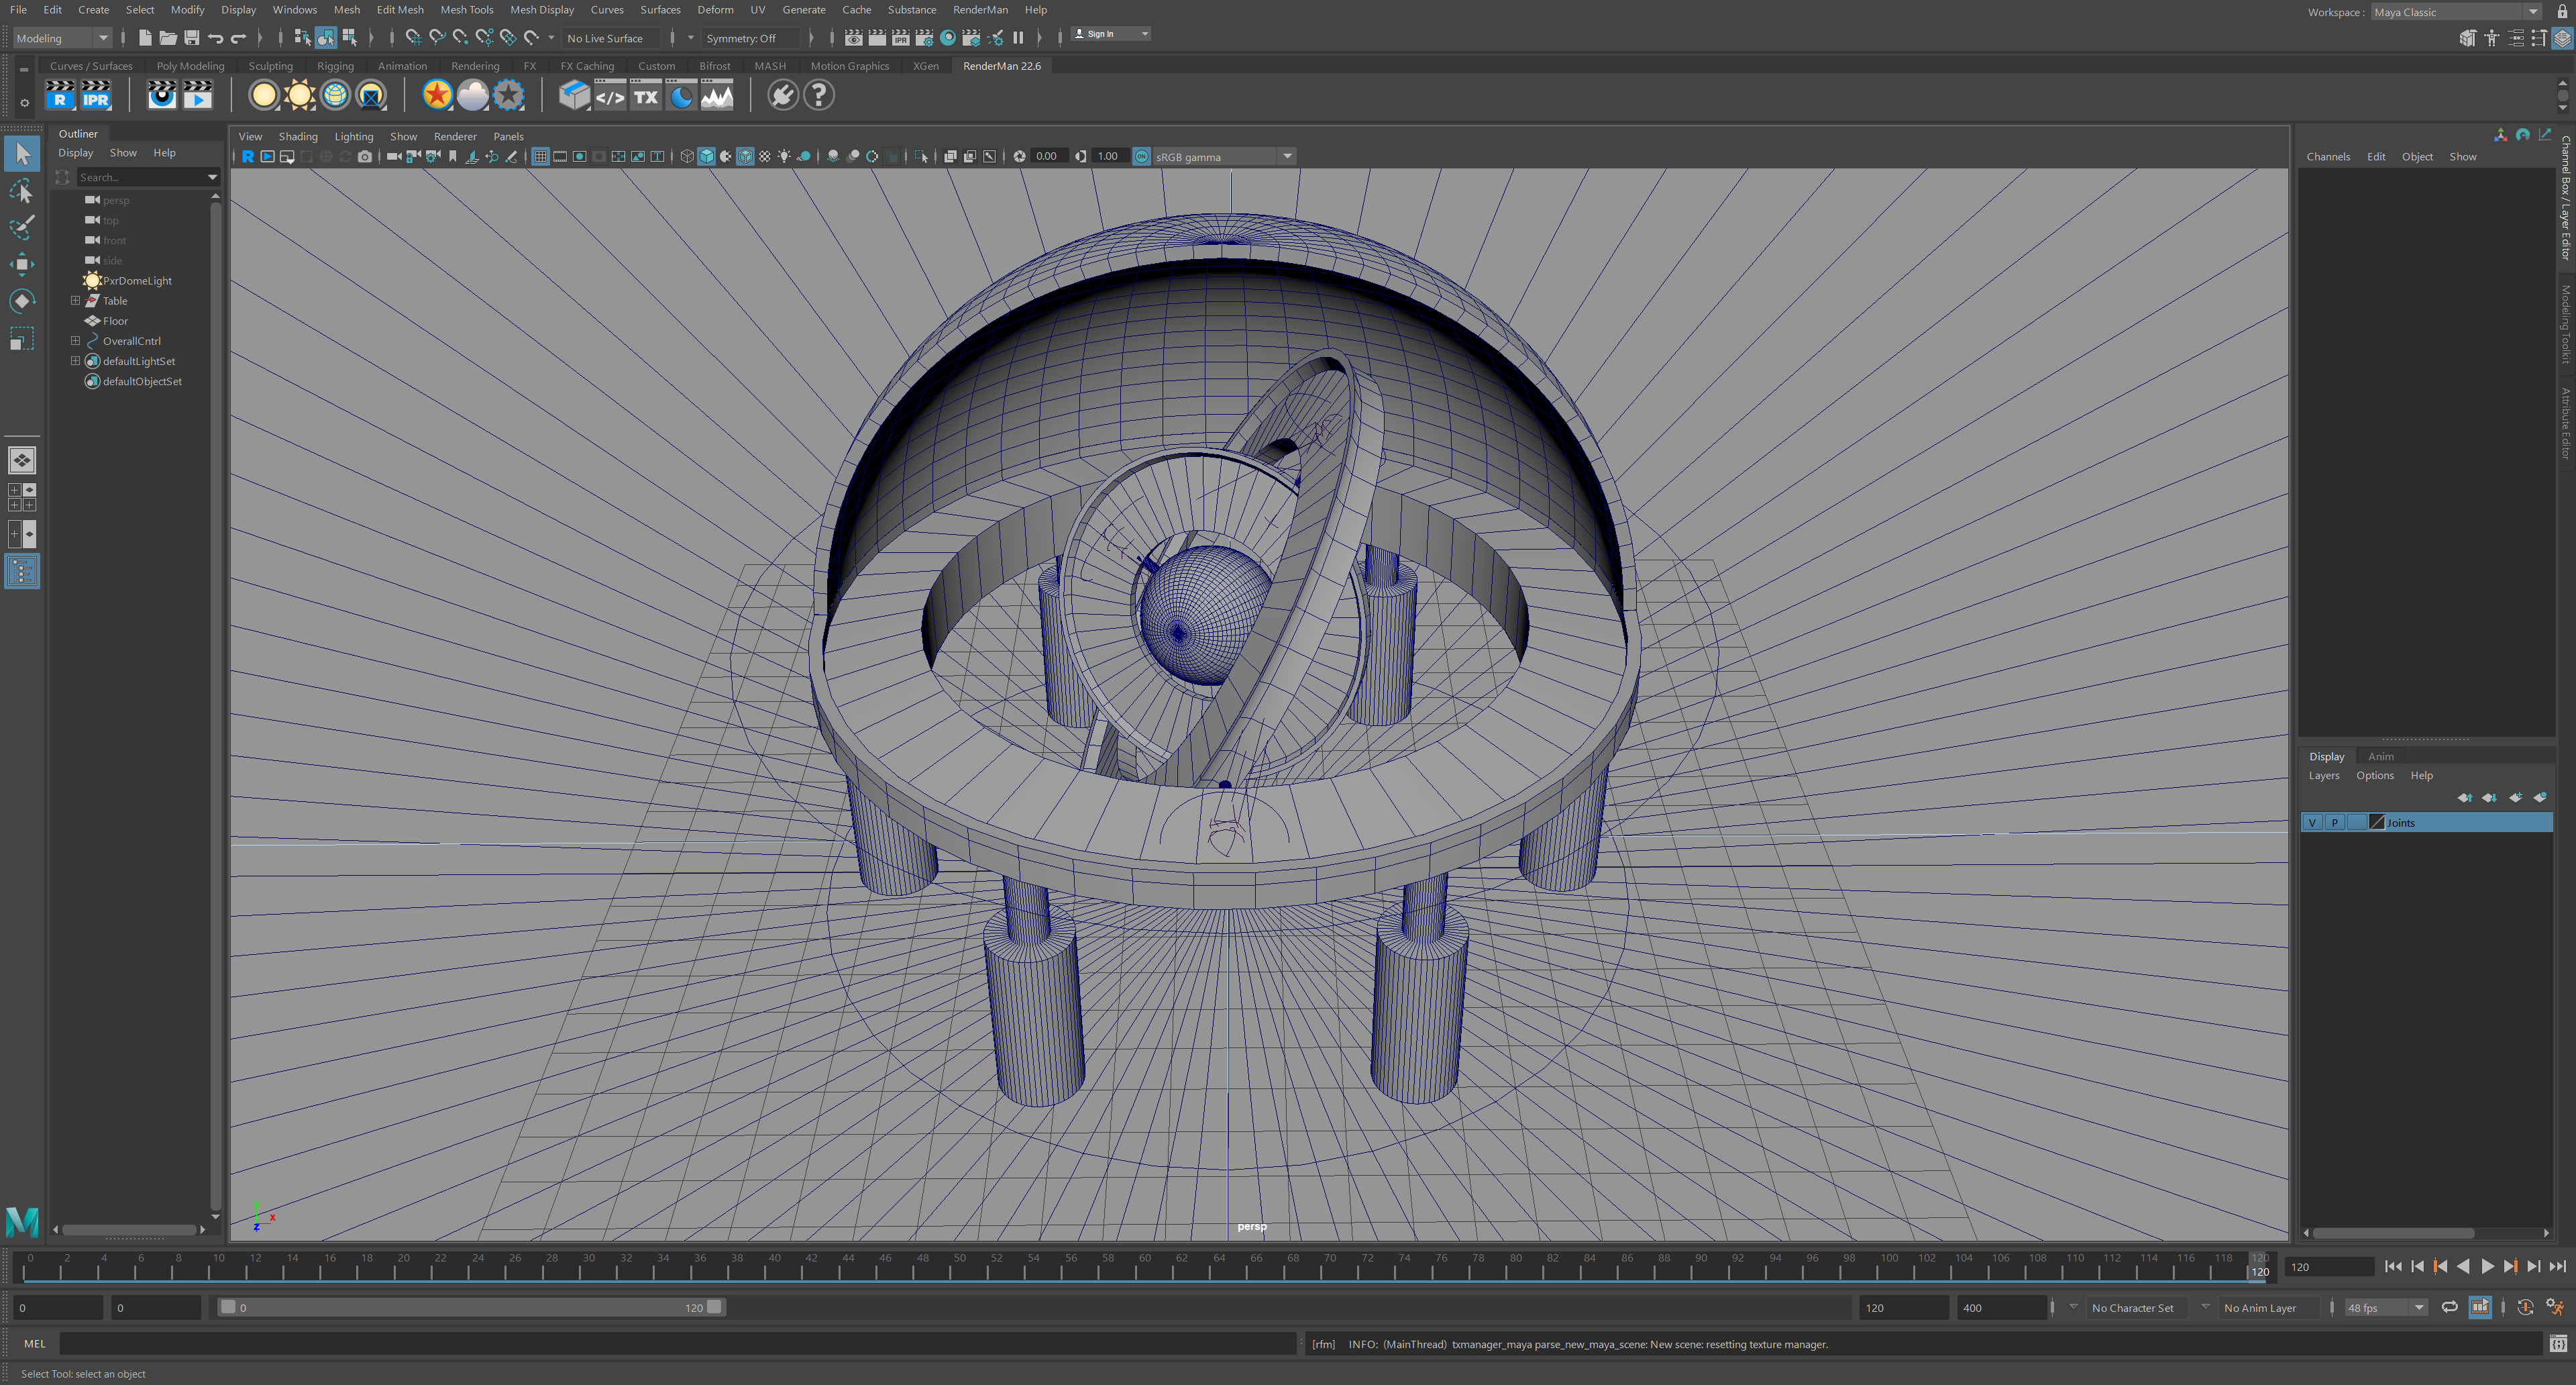
\includegraphics[width=8cm]{project1.png}}
\caption{``Table'' source in Autodesk Maya.}
\label{fig:environment}
\end{minipage}
\end{center}
\end{subfigure}
\par\bigskip
\begin{subfigure}{.5\textwidth}
\begin{center}
\begin{minipage}[t]{\linewidth}
\centerline{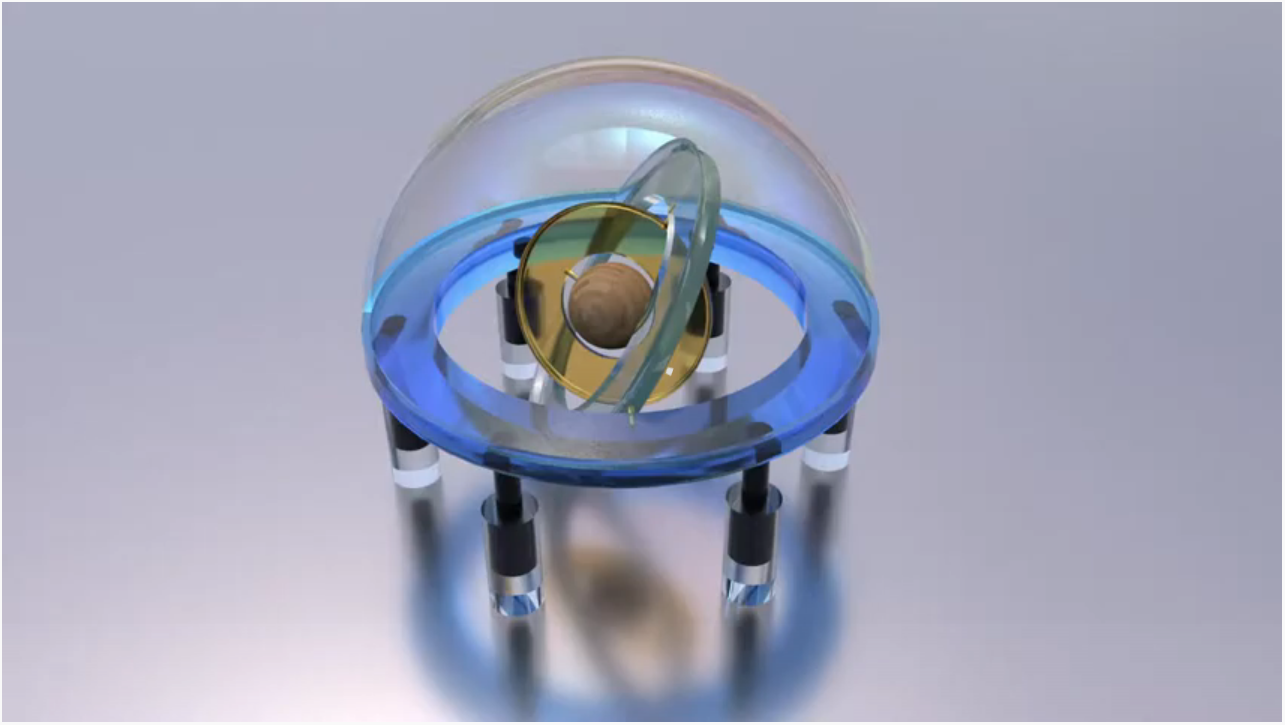
\includegraphics[width=8cm]{table.png}}
\caption{``Table'' rendered with RenderMan \cite{animation}.}
\label{fig:table}
\end{minipage}
\end{center}
\end{subfigure}
\caption{Autodesk Maya and RenderMan environments.}
\label{fig:table_pair}
\end{figure}

Many materials were experimented with. As discussed in \cite{renderman},
RenderMan comes with a shelf of unique material presets that may be further customized as desired.
Instead of choosing one to customize for each part of the table,
many different materials were used in order to obtain the most dynamic render possible.
All components besides the floor and center sphere were transparent, with varying indices of refraction.
The result was a complex scene with a considerably long render-time.
Rendering a single HD (1920 x 1080) frame took around 15 minutes to complete.

\subsection{Animation}
In order to animate the scene, joints were placed at each hinge and parented to the object groups they operate.
Control objects were then created and constrained for each joint group,
so that the joints themselves were left unaltered throughout animation \cite{rigging}.
In total, 5 control objects were used to animate the joints in the scene.
Keyframes were added over the course of 120 frames, and made to loop smoothly.

Since rendering a frame takes about 15 minutes,
rendering the entire 120 frame sequence took approximately 30 hours to complete.
Each frame was then placed into a slideshow and exported in movie format at 30 frames per second.
This created an animation around 5 seconds long,
but with plenty of movement and dynamic material interaction.
One of the final rendered frames of the animated sequence is shown in Figure \ref{fig:table}.
The animation itself is posted on YouTube \cite{animation}.

\section{Implementation}
Here we construct a system architecture to be used for semantics generation.
We decided to implement a system where the objects inside of each frameblock
are extracted from it at runtime, so that semantics for the frameblock
can be generated. We also propose a method of storing this information
in a visual way, to be used in post-processing and keep the render pipeline free from
unnecessary frameblock calculations.
The concept is called ``screen segmentation'', and is described
in detail below.

\subsection{Screen Segmentation}
\begin{figure}[h!]
\begin{center}
\begin{minipage}[t]{\linewidth}
\hspace{0.05\linewidth}
%\rule[-1em]{0pt}{3cm}
\begin{tikzpicture}
% R
\draw (-2,3) -- (3,3); % r horizontal line
\draw (-2,2.95) -- (-2,3.05); % r left tick
\draw (3,2.95) -- (3,3.05); % r right tick
\node[above = 1mm of {(0.5,3)}] {$r$};
%\filldraw[draw=black,fill=lightgray] (1.5,4) rectangle (3.5,4.5);
\filldraw[draw=black,fill={0,0,0}] (-2,1) rectangle (-1,2);
\filldraw[draw=black,fill={1,0,0}] (-1,1) rectangle (0,2);
%\filldraw[draw=black,fill=white] (0,1) rectangle (1,2);
\filldraw[draw=black,fill={6,0,0}] (1,1) rectangle (2,2);
\filldraw[draw=black,fill={7,0,0}] (2,1) rectangle (3,2);
\node[above = 3mm of {(-1.5,2)}] {\scriptsize{$r(1)$}};
\node[above = 0.5mm of {(-1.5,2)}] {\scriptsize{$\textbf{0x01}$}};
\node[above = 3mm of {(-0.5,2)}] {\scriptsize{$r(2)$}};
\node[above = 0.5mm of {(-0.5,2)}] {\scriptsize{$\textbf{0x02}$}};
\node[above = 3mm of {(1.5,2)}] {\scriptsize{$r(7)$}};
\node[above = 0.5mm of {(1.5,2)}] {\scriptsize{$\textbf{0x040}$}};
\node[above = 3mm of {(2.5,2)}] {\scriptsize{$r(8)$}};
\node[above = 0.5mm of {(2.5,2)}] {\scriptsize{$\textbf{0x80}$}};
% B
\draw (-3.25,2) -- (-3.25,-1); % b vertical line
\draw (-3.3,2) -- (-3.2,2); % b top tick
\draw (-3.3,-1) -- (-3.2,-1); % b bottom tick
\node[left = 2mm of {(-3.15,0.5)}] {$b$};
\filldraw[draw=black,fill={0,0,7}] (-2,-1) rectangle (-1,0);
\filldraw[draw=black,fill={1,0,7}] (-1,-1) rectangle (0,0);
%\filldraw[draw=black,fill=white] (0,-1) rectangle (1,0);
\filldraw[draw=black,fill={6,0,7}] (1,-1) rectangle (2,0);
\filldraw[draw=black,fill={7,0,7}] (2,-1) rectangle (3,0);
\node[left = 1mm of {(-2,1.69)}] {\scriptsize{$b(1)$}};
\node[left = 1mm of {(-2,1.36)}] {\scriptsize{$\textbf{0x01}$}};
\node[left = 1mm of {(-2,-0.36)}] {\scriptsize{$b(8)$}};
\node[left = 1mm of {(-2,-0.69)}] {\scriptsize{$\textbf{0x80}$}};
% Dots
\node[right = 1.75mm of {(0,1.5)}] {$\dots$};
\node[right = 1.75mm of {(0,-0.55)}] {$\dots$};
\node[right = 3mm of {(2,0.6)}] {$\vdots$};
\node[right = 3mm of {(-2,0.6)}] {$\vdots$};
\node[right = -3.5mm of {(0.5,0.6)}] {$\ddots$};
% Labels
\node[left = -2mm of {(-1.5,1.5)},fill=white] {$0$};
\node[left = -2mm of {(-0.5,1.5)},fill=white] {$1$};
\node[left = -2mm of {(1.5,1.5)},fill=white] {$6$};
\node[left = -2mm of {(2.5,1.5)},fill=white] {$7$};
\node[left = -2.75mm of {(-1.5,-0.5)},fill=white] {$56$};
\node[left = -2.75mm of {(-0.5,-0.5)},fill=white] {$57$};
\node[left = -2.95mm of {(1.5,-0.5)},fill=white] {$62$};
\node[left = -2.95mm of {(2.5,-0.5)},fill=white] {$63$};
\end{tikzpicture}
\caption{Parameterization of screen space using $r$ and $b$.}
\label{fig:parameterization}
\end{minipage}
\end{center}
\end{figure}

Screen segmentation uses the view of the camera to separate images into different
frameblocks.
In order to export this information visually, we exploit the
red ($r$), green ($g$), and blue ($b$) color channels of an image.
The underlying principle we would like to have in our semantics render,
is a unique color for each object based upon which frameblocks it resides in.
A primitive segmentation of screen space is represented in Figure \ref{fig:parameterization}.
Here $r$ and $b$ were used to parameterize the entire screen
and create a map of colors to frameblocks.
%However there is a problem with the current method of parameterization
%and output color -- it is unknown which frameblocks make up the color
%for a given object.
%These objects have the same frameblock color, even though
%some of the frameblocks are different.
%The discrepency comes from using addition over the space of real values between 0 and 1;
%$1 + 2 + 3$ equals $6$, but so does $3 + 3$. We need a way to uniquely map objects to a given frameblock.
We utilize binary as a means for assigning these values.
Each frameblock is given a unique binary color mask based on its position
in the segemented screen.
The process of screen sementation is outlined below.
Colors can range over 256 values, or 8 bits.
Let each of the 8 x 8 blocks parameterized by $r$ and $b$ each represent one bit,
as shown in Figure \ref{fig:parameterization}
Then each frameblock has a unique color-code with values of 0x01, 0x02, \dots, 0x04, 0x08.
We can use a logical disjunction to ``add'' blocks together, for when
an object resides in more than one frameblock.
The result of this is a unique color for the object representing which frameblocks contain it.

The problem we have now is that the screen can only be broken into 64 blocks.
Since our frames have a screen resolution of 1080 x 1920, this means each block will have
a resolution of 135 x 240. The desired resolution is much smaller, 64 x 64
or even 32 x 32.
This is where we take advantage of the third color channel, $g$.
We can use $g$ to help us break the frame into smaller frameblocks.
Consider using each of the 8 bits of $g$ to overlap with one parameterized section of screen space.
Then the screen can be broken into 4 x 8 x 16 = 512 frameblocks,
so that each frameblock has a resolution of 67 x 60.

This has the desired resolution,
however we find there is yet another problem --
if an object spans multiple 8 x 8 frameblock sections
(the odds of which increases the smaller the frameblocks become),
then it is ambiguous which frameblocks are active and which aren't.
To demonstrate this, consider an object that is contained by 2 frameblocks
and is straddling a frameblock section, as show in Figure \ref{fig:object}.
The object would be thought to be in a frameblock that it is not a part of.
%From the given values of parameterization, the object would have the ultimate
%color code calculated below.
%
%\begin{align*}
%v &= (r = \text{0x80} \wedge \text{0x01},g=\text{0x01} \wedge \text{0x02}, b=\text{0x04} \wedge \text{0x04})\\
%  &= (r=\text{0x81},g=\text{0x03},b=\text{0x04})
%\end{align*}
%
%The only color masks shared between the sections are
%$b = \text{0x04}$, and $b = \text{0x08}$.
%The object's color, however, indicates that
%in sections $g = \text{0x01}$ and $g = \text{0x02}$,
%blocks with red coordinates $(r=\text{0x80},\text{0x10})$ and blue
%$b=\text{0x04},\text{0x08}$ are active.
%Thus, it appears as though the object occupies all eight blocks instead of four.

This dilemma can be solved by offsetting the domains of $g$ so that,
instead of covering frameblocks
$r_i(0..8),b_i(0..8)$,
it covers $r_i(0..4),b_i(0..4)$.
Each 4 x 4 frameblock section has some wiggle-room built in around it,
and therefore has more precision.
The final partition of the screen is shown in Figure \ref{fig:partition}.

\begin{figure}[h!]
\begin{center}
\begin{minipage}[t]{\linewidth}
\hspace{0.065\linewidth}
%\rule[-1em]{0pt}{0cm}
\begin{tikzpicture}
% R
\draw (-2,3) -- (0,3); % r horizontal line
\draw (-2,2.95) -- (-2,3.05); % r left tick
\draw (0,2.95) -- (0,3.05); % r right tick
\node[above = 1mm of {(-1,3)}] {$r(1..8)$};
\draw (0,3) -- (2,3); % r horizontal line
\draw (0,2.95) -- (0,3.05); % r left tick
\draw (2,2.95) -- (2,3.05); % r right tick
\node[above = 1mm of {(1,3)}] {$r(1..8)$};
%\filldraw[draw=black,fill={0,0,0}] (-2,1) rectangle (-1,2);
%\filldraw[draw=black,fill={0,1,0}] (-1,1) rectangle (0,2);
%\filldraw[draw=black,fill={0,2,0}] (0,1) rectangle (1,2);
%\filldraw[draw=black,fill={0,3,0}] (1,1) rectangle (2,2);
\node[above = 3mm of {(-1.5,2)}] {\scriptsize{$g(1)$}};
\node[above = 0.5mm of {(-1.5,2)}] {\scriptsize{$\textbf{0x01}$}};
\node[above = 3mm of {(-0.5,2)}] {\scriptsize{$g(2)$}};
\node[above = 0.5mm of {(-0.5,2)}] {\scriptsize{$\textbf{0x02}$}};
\node[above = 3mm of {(0.5,2)}] {\scriptsize{$g(3)$}};
\node[above = 0.5mm of {(0.5,2)}] {\scriptsize{$\textbf{0x04}$}};
\node[above = 3mm of {(1.5,2)}] {\scriptsize{$g(4)$}};
\node[above = 0.5mm of {(1.5,2)}] {\scriptsize{$\textbf{0x08}$}};
% B
\draw (-2.25,2) -- (-2.25,0); % b vertical line
\draw (-2.3,2) -- (-2.2,2); % b top tick
\draw (-2.3,0) -- (-2.2,0); % b bottom tick
\node[left = 2mm of {(-2.15,1)}] {$b(1..8)$};
%\filldraw[draw=black,fill={0,4,0}] (-2,0) rectangle (-1,1);
%\filldraw[draw=black,fill={0,5,0}] (-1,0) rectangle (0,1);
%\filldraw[draw=black,fill={0,6,0}] (0,0) rectangle (1,1);
%\filldraw[draw=black,fill={0,7,0}] (1,0) rectangle (2,1);
\shade[left color={7,0,1},right color={1,0,7}, shading angle=-45] (-2,1) rectangle (-1,2);
%\shade[path fading=rectangular fading, fill={7,0,7}] (-2,1) rectangle (-1,2);
\shade[left color={7,1,1},right color={1,1,7}, shading angle=-45] (-1,1) rectangle (0,2);
%\shade[path fading=rectangular fading, fill={7,0,7}] (-1,1) rectangle (0,2);
\shade[left color={7,2,1},right color={1,2,7}, shading angle=-45] (0,1) rectangle (1,2);
%\shade[path fading=rectangular fading, fill={7,0,7}] (0,1) rectangle (1,2);
\shade[left color={7,3,1},right color={1,3,7}, shading angle=-45] (1,1) rectangle (2,2);
%\shade[path fading=rectangular fading, fill={7,0,7}] (1,1) rectangle (2,2);
\shade[left color={7,4,1},right color={1,4,7}, shading angle=-45] (-2,0) rectangle (-1,1);
\shade[left color={7,5,1},right color={1,5,7}, shading angle=-45] (-1,0) rectangle (0,1);
\shade[left color={7,6,1},right color={1,6,7}, shading angle=-45] (0,0) rectangle (1,1);
\shade[left color={7,7,1},right color={1,7,7}, shading angle=-45] (1,0) rectangle (2,1);

\node[below = 0.5mm of {(-1.5,0)}] {\scriptsize{$g(5)$}};
\node[below = 3mm of {(-1.5,0)}] {\scriptsize{$\textbf{0x10}$}};
\node[below = 0.5mm of {(-0.5,0)}] {\scriptsize{$g(6)$}};
\node[below = 3mm of {(-0.5,0)}] {\scriptsize{$\textbf{0x20}$}};
\node[below = 0.5mm of {(0.5,0)}] {\scriptsize{$g(7)$}};
\node[below = 3mm of {(0.5,0)}] {\scriptsize{$\textbf{0x40}$}};
\node[below = 0.5mm of {(1.5,0)}] {\scriptsize{$g(8)$}};
\node[below = 3mm of {(1.5,0)}] {\scriptsize{$\textbf{0x80}$}};
% Labels
\node[left = -3mm of {(-1.5,1.5)},fill=white] {$64$};
\node[left = -3.5mm of {(-0.5,1.5)},fill=white] {$128$};
\node[left = -3.5mm of {(0.5,1.5)},fill=white] {$192$};
\node[left = -3.75mm of {(1.5,1.5)},fill=white] {$256$};
\node[left = -3.75mm of {(-1.5,0.5)},fill=white] {$320$};
\node[left = -3.75mm of {(-0.5,0.5)},fill=white] {$384$};
\node[left = -3.8mm of {(0.5,0.5)},fill=white] {$448$};
\node[left = -3.85mm of {(1.5,0.5)},fill=white] {$512$};
\end{tikzpicture}
\caption{Final partition of screen space, where $g$ on top of the $r$ and $b$ parameterization.}
\label{fig:partition}
\end{minipage}
\end{center}
\end{figure}

The usecase would then be to test the value of $g$ before evaluating $r$ and $b$.
This solution divides the domains of $g$ in half,
meaning we can only cover 128 frameblocks instead of 512, and blocks now have
resolutions of 135 x 120.
An example calculation of the final segmentation system is shown in Figure \ref{fig:example}.
This proves that, although there are less frameblocks, the accuracy of the colors increases for objects spanning frameblock sections.

\begin{figure}[h!]
\centering
\begin{subfigure}{.5\textwidth}
\begin{center}
\begin{minipage}[t]{\linewidth}
\hspace{-0.025\linewidth}
\begin{tikzpicture}
% G
\draw (-3.375,1.9) -- (0,1.9); % g horizontal line
\draw (-3.375,1.85) -- (-3.375,1.95); % g left tick
\draw (0,1.85) -- (0,1.95); % g right tick
\node[above = 0.5mm of {(-1.6875,1.9)}] {$g(6)$};
\draw (0,1.9) -- (3.375,1.9); % g horizontal line
\draw (0,1.85) -- (0,1.95); % g left tick
\draw (3.375,1.85) -- (3.375,1.95); % g right tick
\node[above = 0.5mm of {(1.6875,1.9)}] {$g(7)$};
\filldraw[draw=black,fill={0,4,0}] (-3.375,-1.6875) rectangle (0,1.6875);
\filldraw[draw=black,fill={0,6,0}] (0,-1.6875) rectangle (3.375,1.6875);
% R
\draw (-3,-1.9) -- (-0.375,-1.9); % r horizontal line
\draw (-3,-1.85) -- (-3,-1.95); % r left tick
\draw (-0.375,-1.85) -- (-0.375,-1.95); % r right tick
\node[below = -0.5mm of {(-1.6875,-1.9)}] {$r(3,4)$};
\draw (0.375,-1.9) -- (3,-1.9); % r horizontal line
\draw (0.375,-1.85) -- (0.375,-1.95); % r left tick
\draw (3,-1.85) -- (3,-1.95); % r right tick
\node[below = -0.5mm of {(1.6875,-1.9)}] {$r(5,6)$};
% B
\draw (-3.6,-1.3125) -- (-3.6,1.3125); % b vertical line
\draw (-3.55,1.3125) -- (-3.65,1.3125); % b top tick
\draw (-3.55,-1.3125) -- (-3.65,-1.3125); % b bottom tick
\node[left = 0mm of {(-3.6,0)}] {$b(3,4)$};
% Left pairs
\filldraw[draw=black,fill={0,4,2}] (-3,-1.3125) rectangle (-1.6875,0); % bottom left
\filldraw[draw=black,fill={0,4,4}] (-1.6875,-1.3125) rectangle (-0.375,1.3125); % bottom right
\filldraw[draw=black,fill={2,4,0}] (-3,0) rectangle (-1.6875,1.3125); % top left
\filldraw[draw=black,fill={4,4,0}] (-1.6875,0) rectangle (-0.375,1.3125); % top right
% Right pairs
\filldraw[draw=black,fill={0,6,2}] (0.375,-1.3125) rectangle (1.6875,0); % bottom left
\filldraw[draw=black,fill={0,6,4}] (1.6875,-1.3125) rectangle (3,1.3125); % bottom right
\filldraw[draw=black,fill={2,6,0}] (0.375,0) rectangle (1.6875,1.3125); % top left
\filldraw[draw=black,fill={4,6,0}] (1.6875,0) rectangle (3,1.3125); % top right
% Object
\filldraw[draw=black,fill={8,8,8},fill opacity=0.25] (0,0) circle (3em);
\pattern [pattern=checkerboard,pattern color={8,8,8}] (0,0) circle (3em);
\end{tikzpicture}
\caption{Example of an object overlapping a partition}
\label{fig:object}
\end{minipage}
\end{center}
\end{subfigure}
\par\bigskip
\begin{subfigure}{.5\textwidth}
\begin{center}
\begin{minipage}[t]{\linewidth}
\hspace{0.225\linewidth}
\begin{tikzpicture}
% Squares
\filldraw[draw=black,fill={4,4,0}] (-2.5,1) rectangle (2.5,2); % top left
\filldraw[draw=black,fill={2,6,0}] (-2.5,0) rectangle (2.5,1); % top right
\filldraw[draw=black,fill={0,6,4}] (-2.5,-1) rectangle (2.5,0); % bottom left
\filldraw[draw=black,fill={0,6,2}] (-2.5,-2) rectangle (2.5,-1); % bottom right
\draw[dashed] (-2.5,-2.5) -- (2.5,-2.5); % horizontal line
\filldraw[draw=black,fill={8,8,8}] (-2.5,-4) rectangle (2.5,-3); % bottom right
% Labels
\node[above = -3mm of {(0,1.5)},fill=white] {\small$(r,g,b)=\text{(0x08,0x20,0x04)}$}; % top
\node[above = -3mm of {(0,0.5)},fill=white] {\small$(r,g,b)=\text{(0x08,0x40,0x08)}$};
\node[above = -3mm of {(0,-0.5)},fill=white] {\small$(r,g,b)=\text{(0x10,0x20,0x04)}$};
\node[above = -3mm of {(0,-1.5)},fill=white] {\small$(r,g,b)=\text{(0x10,0x40,0x08)}$};
% Ops
\node[right = 3mm of {(2.5,1.5)},fill=white] {\large$\mathbf{\oplus}$};
\node[right = 3mm of {(2.5,0.5)},fill=white] {\large$\mathbf{\oplus}$};
\node[right = 3mm of {(2.5,-0.5)},fill=white] {\large$\mathbf{\oplus}$};
\node[right = 3mm of {(2.5,-1.5)},fill=white] {\large$\mathbf{\oplus}$};
\node[right = 3mm of {(2.5,-2.5)},fill=white] {\large$\mathbf{=}$};
% Object
\node[above = -3mm of {(0,-3.5)},fill=white] {\small$(r,g,b)=\text{(0x18,0x60,0x0B)}$};
\end{tikzpicture}
\caption{Derivation of the color for the example object.}
\label{fig:object_color}
\end{minipage}
\end{center}
\end{subfigure}
\caption{Example showing how a color is selected for an object straddling more than one frameblock.
The color of the circle is made up of the logical disjunction of color bits.}
\label{fig:example}
\end{figure}

\subsection{Optimizations and Other Considerations}
While the 8-bit model proved useful for integer storage of color values,
there are other models that have more precision than 8 bits.
Using floating-point values, we can have up to 64 bits of precision.
While this is fine in theory, the increased precision can make it harder to distinguish
objects from each other at runtime.

Renders for both 8-bit and 16-bit precision are shown in
Figure \ref{fig:render_comparisons}.
From comparing the two, it is clear that 8-bit precision offers a clearer representation
of the color spectrum than the 16-bit model.
This is by nature of binary, since color values are halved with each successive bit.
We can however use the 16-bit color values given precise enough color detection
or if the shaders that they are stored in are available.
If neither option exists, the only possibility is to use the 8-bit precision,
with 135 x 120 resolution frameblocks.

\subsection{Final Semantics Generation}
Now that we have found a way to find if an is object inside of a frameblock,
we must decide what data on that object to collect and export.
The visual representation of relationship of objects and screen space
is not enough semantics data for training machine learning alogrithms.
If we collect enough information about each object,
we should be able to discern some amount of clarity
for how that object interacts with others given the frameblock it is in.
The following information for each object is collected:
\bigskip
\begin{enumerate}
\item Distance to center of frameblock.
\item Translation of object.
\item Rotation of object.
\item Scaling of object.
\end{enumerate}
\bigskip

The above data is stored for each object in a frameblock and exported
per frame in JSON format.
Figure \ref{fig:distances} shows an example of collecting
distances of objects relative to a frameblock.
We decided that since the distances of neighboring objects (the dashed lines)
is unchanging for a frame, it would not be productive to include these values.

\begin{adjustwidth}{2.5em}{0pt}
\begin{figure}[h!]
\begin{center}
\begin{tikzpicture}
\coordinate (P) at (3,2);
\coordinate (Q) at (3.5,0);
\coordinate (R) at (2,-1.5);
\draw (-1.25,1) -- (-0.75,1); % Screen (top)
\draw (-1,-1) -- (-1,1); % Screen (Z)
\draw (-1.25,-1) -- (-0.75,-1); % Screen (bottom)
\draw (-1,0) -- (3,1.5); % ZP
\draw (-1,0) -- (3.5,0); % ZQ
\draw (-1,0) -- (2,-1.5); % ZR
\draw[dashed] (3,1.5) -- (2,-1.5); % PR
\draw[dashed] (3,1.5) -- (3.5,0); % PQ
\draw[dashed] (3.5,0) -- (2,-1.5); % QR
%%Labels for the vertices are typeset.
\node[below left = -2.45mm of {(3,1.5)}] {\textbullet}; % P
\node[below left = -2.35mm of {(3.5,0)}] {\textbullet}; % Q
\node[below left = -2.5mm of {(2,-1.5)}] {\textbullet}; % R
\node[right = 1mm of {(3,1.5)}] {$P$};
\node[right = 1mm of {(3.5,0)}] {$Q$};
\node[right = 1mm of {(2,-1.5)}] {$R$};
\node[right = -5mm of {(-1,-1.3)}] {$S_{x,y,z}$};
\end{tikzpicture}
\end{center}
\caption{Relationships between points $P$, $Q$, and $R$ and frameblock with world coordinates $S_{x,y,z}$.}
\label{fig:distances}
\end{figure}
\end{adjustwidth}

We hope that, when paired with the actual render for a frame,
the exported semantics of each frameblock can be used to
learn how to produce a new frame given its semantic data.

\subsection{Results}
A prototype system was constructed using RenderMan
and Python scripting, and applied to a frame of the scene.
New RenderMan nodes each with a custom shader were created for each object in the scene.
These nodes render a constant color, set by $r$, $g$, and $b$ variable inputs.
A Python script was then written in order to set the inputs for each shader.
The script accomplished the following:
\bigskip
\begin{enumerate}
\item Split the screen into a variable number of frameblocks.
\item Transformed all objects in the scene into screen space, using world-to-screen camera transformation.
\item Used the Cohen-Sutherland algorithm to identify if an edge of an object is inside a frameblock.
\item Parameterized screen space as shown in Figure \ref{fig:partition}.
\item Calculated the floating point color value for the centroid of each frameblock.
\item Assigned a color value to each object, where
$F$ is the set of frameblocks the object is inside of:
$$v_{object} = \sum_{v_i\in F}v_i$$
\item Stored the color values for each object in RenderMan shaders.
\end{enumerate}
\bigskip
RenderMan is used to render the encoded frame.
Figure \ref{fig:render_comparisons}
shows the example scene rendered with frameblock encodings.
Both 8-bit and 16-bit precisions are rendered, for visual comparison.

The semantics are then generated.
\bigskip
\begin{enumerate}
\item Collected color values of each object from their shaders.
\item Check if the calculated frameblocks of each object are equal to the ones it
resides in.
\item Loop over all frameblocks
\begin{enumerate}
\item Collect semantic data for all objects visible to each frameblock.
\end{enumerate}
\item Export the collected semantic data in JSON format.
\end{enumerate}

\begin{figure*}[htbp]
\centering
\begin{subfigure}{1.1\textwidth}
\begin{center}
\begin{minipage}[t]{\linewidth}
\hspace{-0.09\linewidth}
  \centering
    \begin{subfigure}{.49\textwidth}
      \centering
      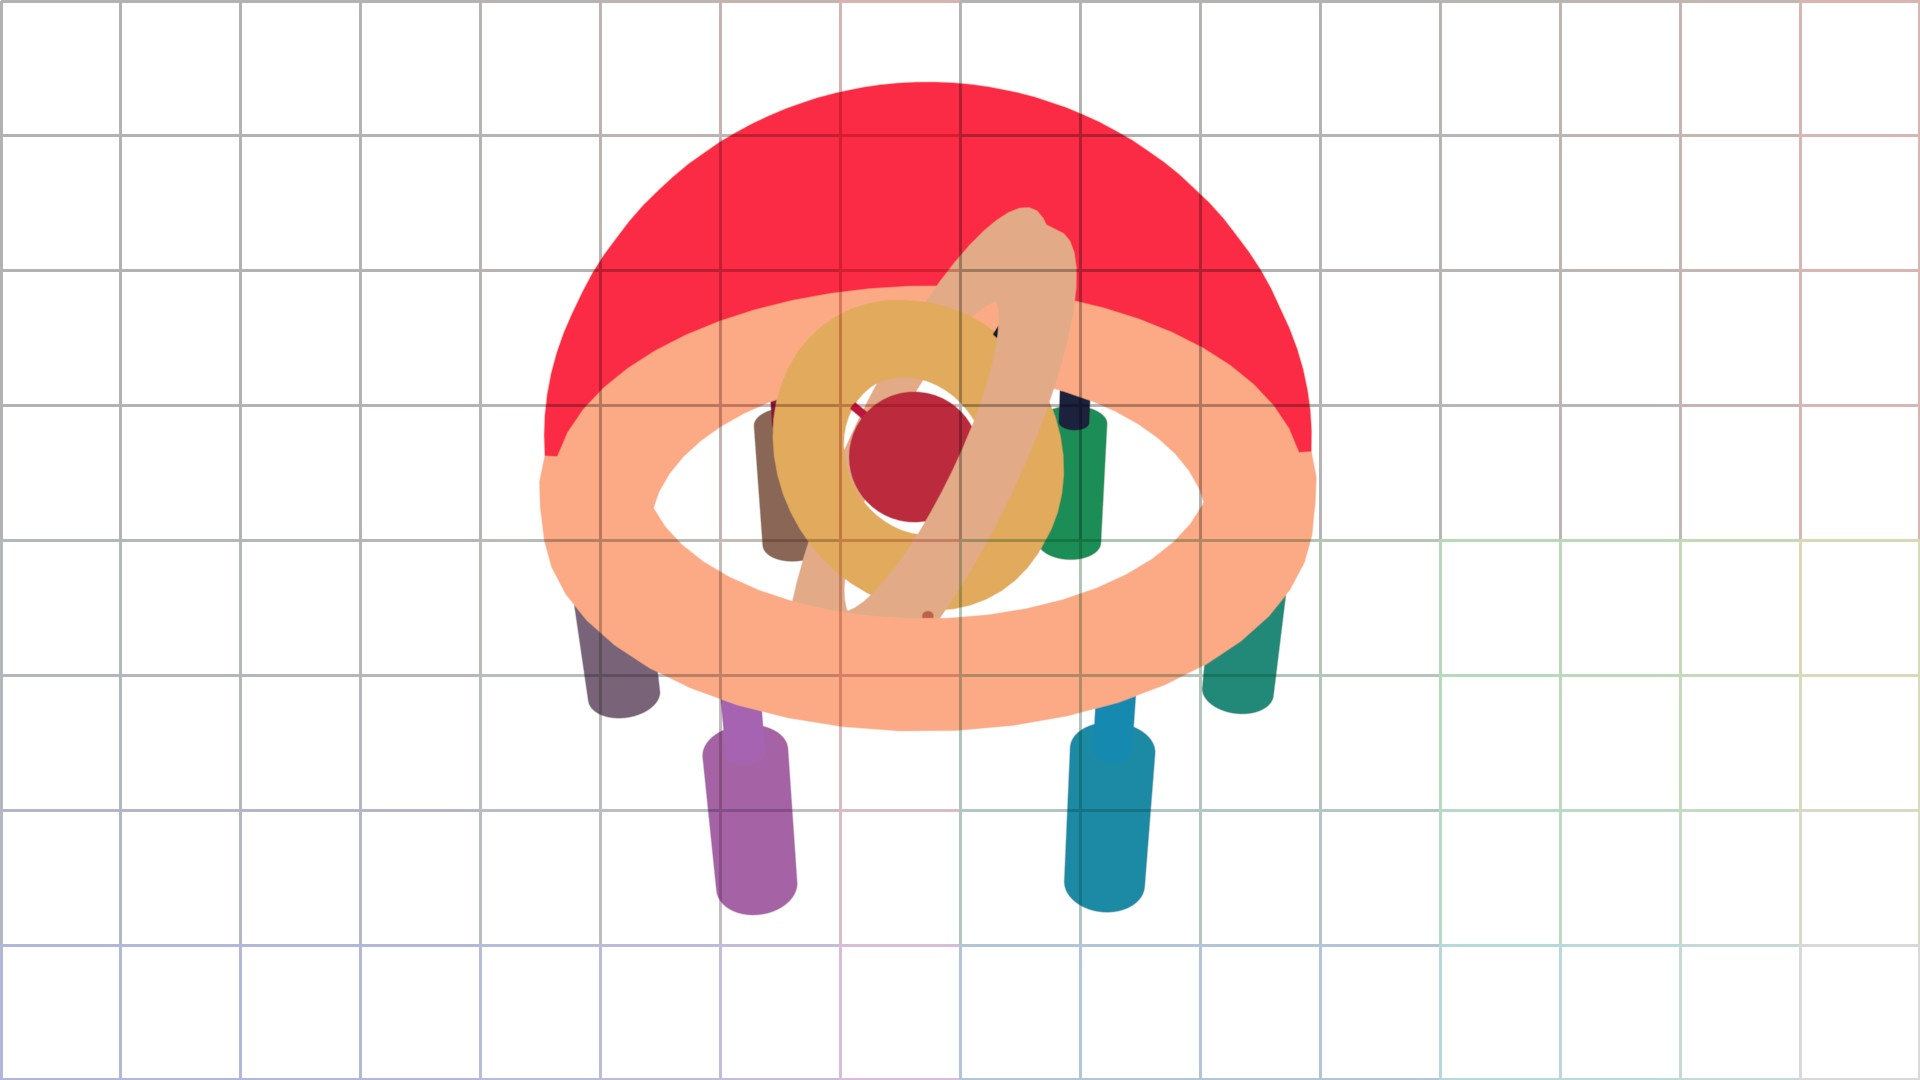
\includegraphics[width=\linewidth]{8_render.jpg}
      \caption{8-bit precision render.}
      \label{fig:render_8}
    \end{subfigure}
    \begin{subfigure}{.49\textwidth}
      \centering
      
\includegraphics[width=\linewidth]{8_partition.jpg}
      \caption{8-bit precision screen partition.}
      \label{fig:render_8}
    \end{subfigure}
  \label{fig:render_8}
\end{minipage}
\end{center}
\end{subfigure}
\par\medskip
\begin{subfigure}{1.1\textwidth}
\begin{center}
\begin{minipage}[t]{\linewidth}
\hspace{-0.09\linewidth}
  \centering
    \begin{subfigure}{.49\textwidth}
      \centering
      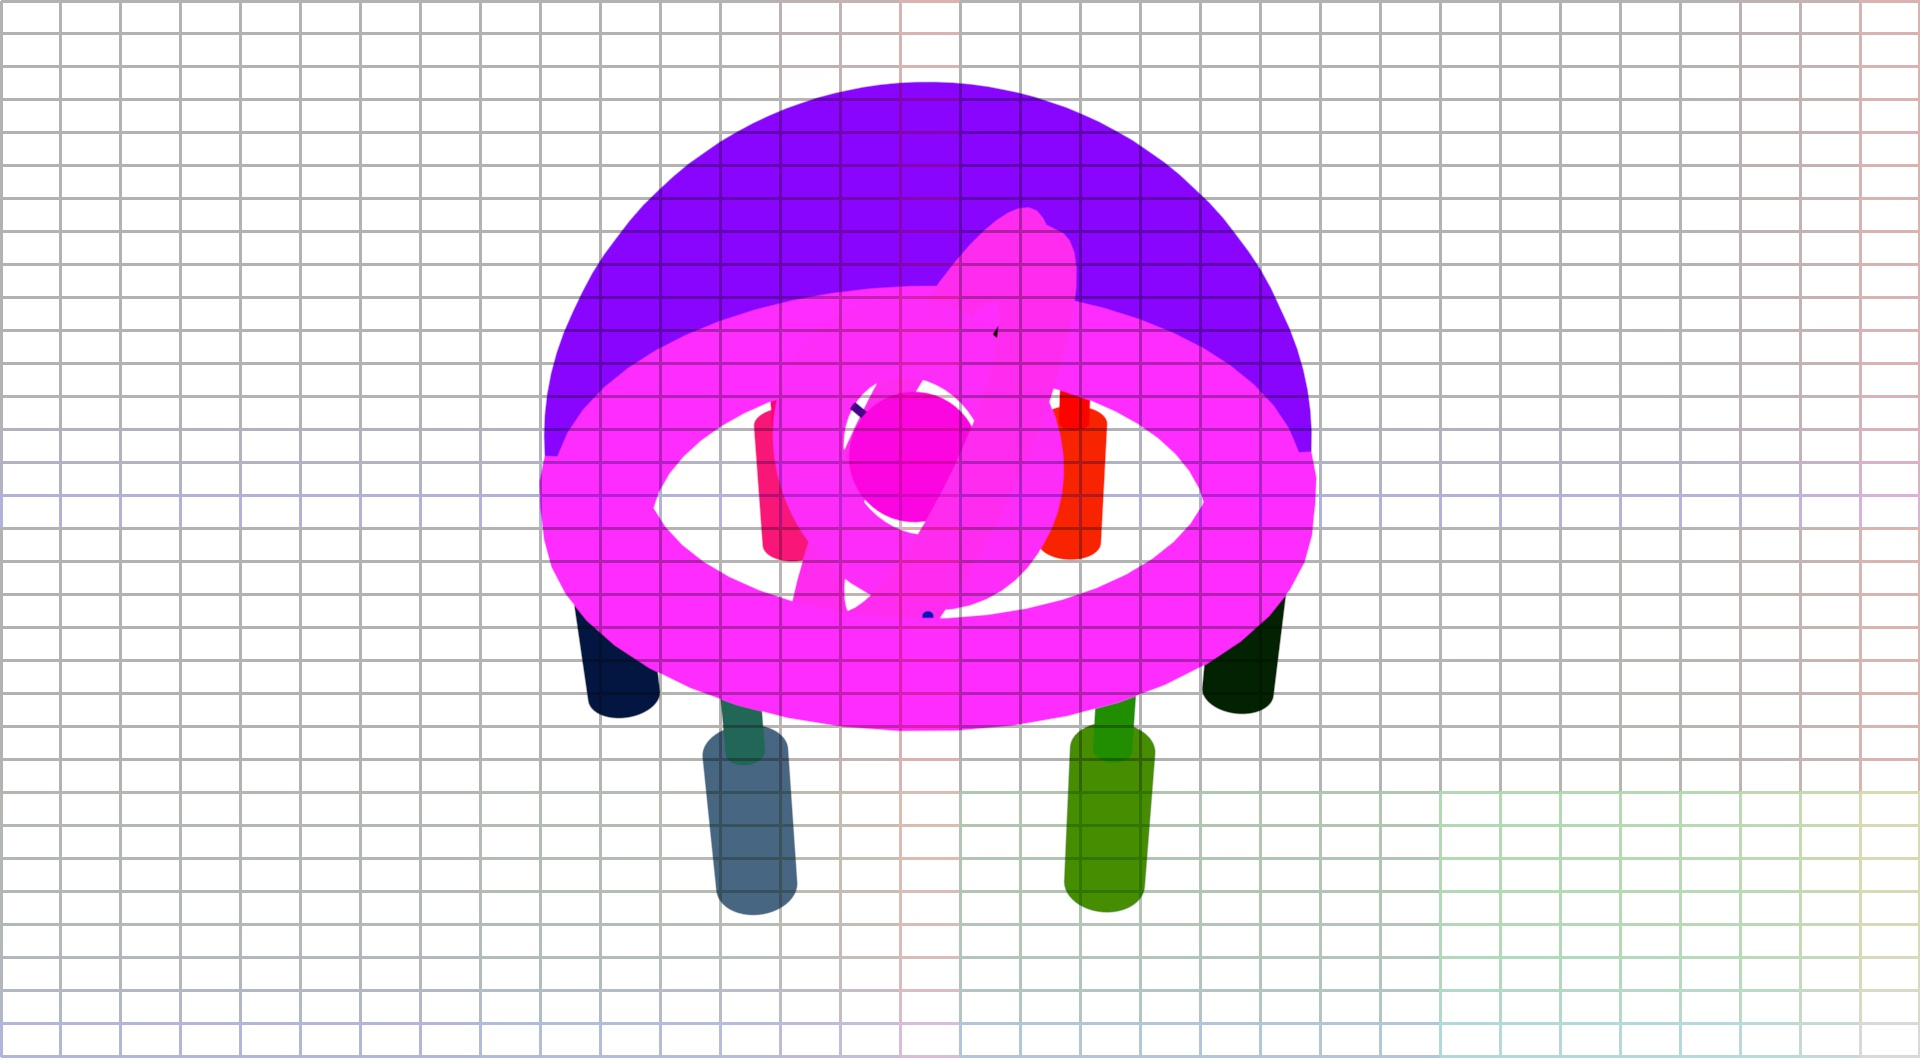
\includegraphics[width=\linewidth]{16_render_cropped.jpg}
      \caption{16-bit precision render.}
      \label{fig:render_8}
    \end{subfigure}
    \begin{subfigure}{.49\textwidth}
      \centering
      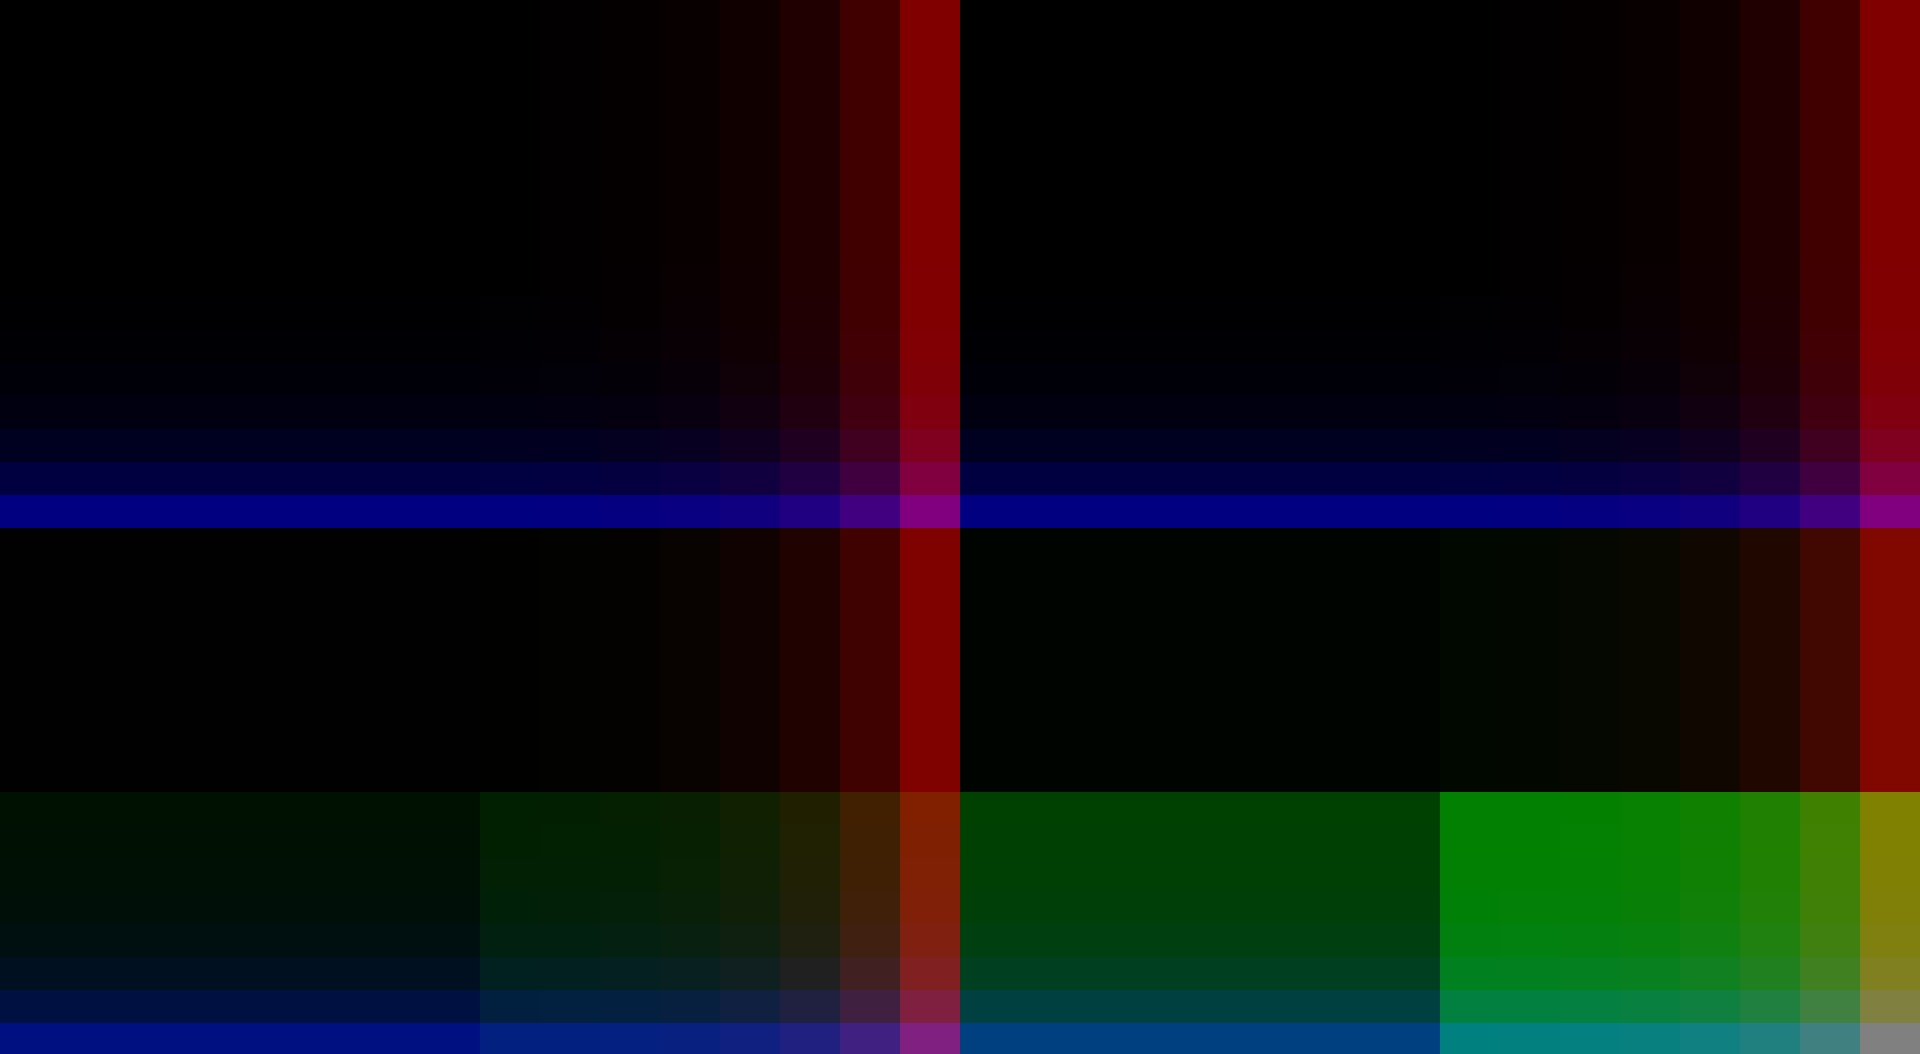
\includegraphics[width=\linewidth]{16_partition_cropped.jpg}
      \caption{16-bit precision screen segmentation.}
      \label{fig:render_8}
    \end{subfigure}
  \label{fig:render_16}
\end{minipage}
\end{center}
\end{subfigure}
\caption{Renders of differing precisions compared to screen space segementation.}
\label{fig:render_comparisons}
\end{figure*}

\section{Conclusion}
\label{sec:conclusion}
A qualifying computer was built, and a basic environment installed.
Then a dynamic scene was animated in Autodesk Maya and exported
using RenderMan. Research into collecting semantics from the scene using
the RenderMan Interface and RenderMan Shading Language (RSL)
will be the focus of the project from now on.

We propose a study of the relationship between objects in a 3D scene and rendered images.
Semantics data is easily recognizable by humans, but much harder for machines.
Automating the process is a complicated task that will involve much consideration over
scene dynamics and the relationship of objects to what is rendered.
Ray tracing is also a concept
key to many difficult tasks, and this project is an
opportunity to explore the implementation of ray tracing and its application
to difficult problems in Computer Graphics.

\bibliography{project}
\bibliographystyle{IEEEtran}

\onecolumn

\pagebreak

\begin{center}
\section*{Appendix}
\label{app:b}
\end{center}

\bigskip

\footnotesize{
\begin{minted}{python}
\end{minted}
%==========================================================
\end{document}
%==========================================================
